\documentclass[tikz, border=15pt]{standalone}
\usepackage{tikz}
\usetikzlibrary{shapes.geometric, calc}

\definecolor{wallcolor}{HTML}{F9F3EA}
\definecolor{floorcolor}{HTML}{DDB892}
\definecolor{rugcolor}{HTML}{E6C280}
\definecolor{sofacolor}{HTML}{B5838D}
\definecolor{tvcolor}{HTML}{333333}
\definecolor{screenlight}{HTML}{E8F1F5}
\definecolor{woodcolor}{HTML}{7F5539}
\definecolor{curtaincolor}{HTML}{E07A5F}
\definecolor{lampglow}{HTML}{F2CC8F}
\definecolor{grandmahair}{HTML}{E0E0E0}
\definecolor{grandmacloth}{HTML}{81B29A}
\definecolor{skincolor}{HTML}{FFDAB9}

\begin{document}
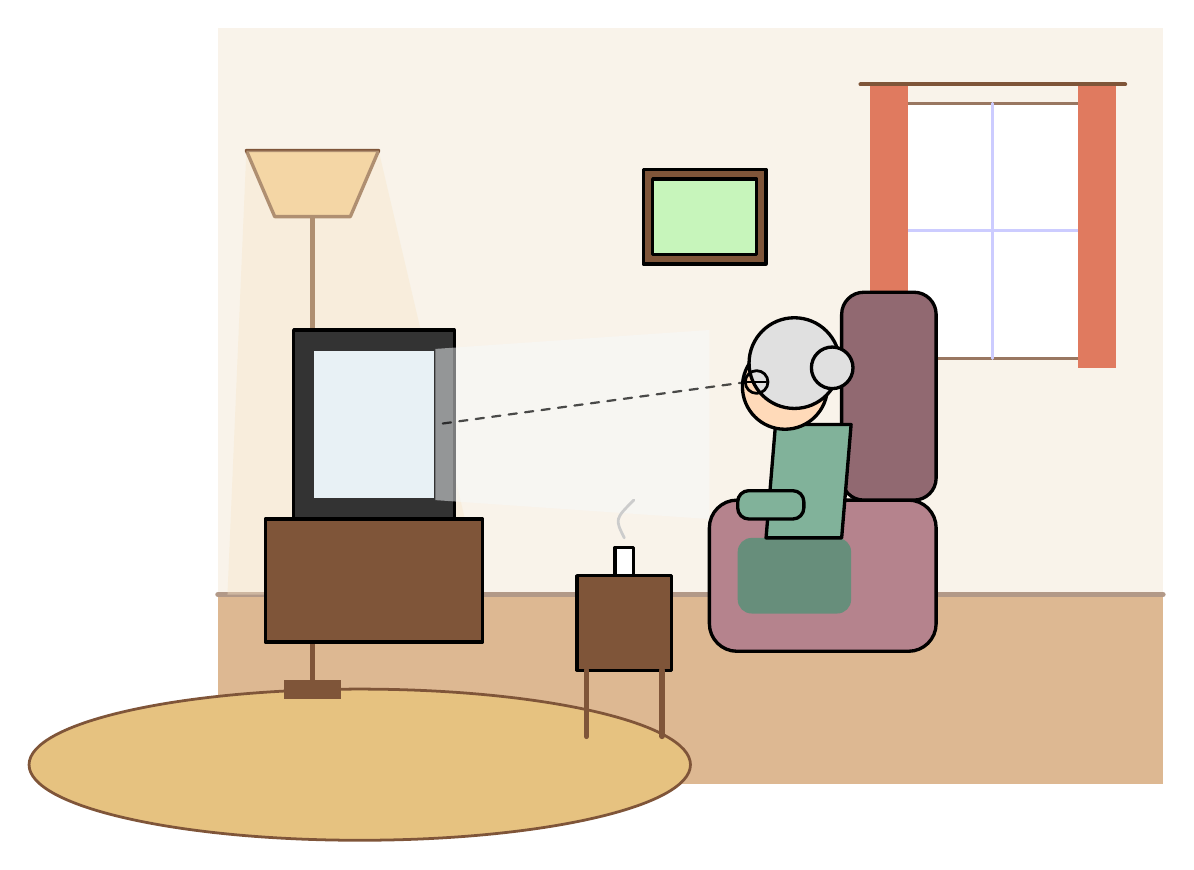
\begin{tikzpicture}[
    scale=1.2,
    line width=1.2pt,
    line join=round,
    line cap=round
]

    % Room Background: Wall and Floor
    \fill[wallcolor] (-5, -2) rectangle (5, 4);
    \fill[floorcolor] (-5, -4) rectangle (5, -2);
    \draw[woodcolor!60, line width=2pt] (-5, -2) -- (5, -2);

    % Cozy Rug
    \fill[rugcolor, draw=woodcolor, line width=1pt] (-3.5, -3.8) ellipse (3.5 and 0.8);

    % Window & Curtain (Right side background)
    \fill[white, draw=woodcolor!80] (2.2, 0.5) rectangle (4.2, 3.2);
    \draw[blue!20, line width=1pt] (2.2, 1.85) -- (4.2, 1.85);
    \draw[blue!20, line width=1pt] (3.2, 0.5) -- (3.2, 3.2);
    \fill[curtaincolor] (1.9, 0.4) rectangle (2.3, 3.4);
    \fill[curtaincolor] (4.1, 0.4) rectangle (4.5, 3.4);
    \draw[woodcolor, line width=1.5pt] (1.8, 3.4) -- (4.6, 3.4);

    % Floor Lamp (Left background)
    \draw[woodcolor, line width=2pt] (-4, -3) -- (-4, 2);
    \fill[woodcolor] (-4.3, -3.1) rectangle (-3.7, -2.9);
    \fill[lampglow, draw=woodcolor] (-4.4, 2) -- (-3.6, 2) -- (-3.3, 2.7) -- (-4.7, 2.7) -- cycle;
    \fill[lampglow!50, opacity=0.4] (-4.7, 2.7) -- (-3.3, 2.7) -- (-2.2, -2) -- (-4.9, -2) -- cycle;

    % TV Console & TV (Left-center side facing right)
    \fill[woodcolor, draw=black] (-4.5, -2.5) rectangle (-2.2, -1.2);
    \fill[tvcolor, draw=black] (-4.2, -1.2) rectangle (-2.5, 0.8);
    \fill[screenlight, draw=tvcolor] (-4.0, -1.0) rectangle (-2.7, 0.6);
    % TV Screen glow rays towards grandma
    \fill[screenlight!40, opacity=0.5] (-2.7, 0.6) -- (-2.7, -1.0) -- (0.2, -1.2) -- (0.2, 0.8) -- cycle;

    % Small Table with Tea Cup in middle
    \fill[woodcolor, draw=black] (-1.2, -2.8) rectangle (-0.2, -1.8);
    \draw[woodcolor, line width=2pt] (-1.1, -3.5) -- (-1.1, -2.8);
    \draw[woodcolor, line width=2pt] (-0.3, -3.5) -- (-0.3, -2.8);
    % Tea Cup
    \fill[white, draw=black] (-0.8, -1.8) rectangle (-0.6, -1.5);
    \draw[white!80!black, line width=1pt] (-0.7, -1.4) .. controls (-0.8, -1.2) .. (-0.6, -1.0); % Steam

    % Armchair / Sofa (Right-center facing left)
    \fill[sofacolor, draw=black, rounded corners=10pt] (0.2, -2.6) rectangle (2.6, -1.0);
    \fill[sofacolor!80!black, draw=black, rounded corners=8pt] (1.6, -1.0) rectangle (2.6, 1.2); % Backrest

    % Grandma sitting on Sofa
    % Lower Body
    \fill[grandmacloth!80!black, rounded corners=5pt] (0.5, -2.2) rectangle (1.7, -1.4);
    % Upper Body
    \fill[grandmacloth, draw=black] (0.8, -1.4) -- (1.6, -1.4) -- (1.7, -0.2) -- (0.9, -0.2) -- cycle;
    % Arm resting on armrest
    \fill[grandmacloth, draw=black, rounded corners=4pt] (0.5, -1.2) rectangle (1.2, -0.9);
    % Head (tilted towards TV on the left)
    \fill[skincolor, draw=black] (1.0, 0.2) circle (0.45);
    % Hair (White/Grey bun)
    \fill[grandmahair, draw=black] (1.1, 0.45) circle (0.48);
    \fill[grandmahair, draw=black] (1.5, 0.4) circle (0.22); % Bun
    % Glasses & Eye sightline
    \draw[black, line width=1pt] (0.7, 0.25) circle (0.12);
    \draw[black, line width=1pt] (0.6, 0.25) -- (0.8, 0.25);
    \draw[black, dashed, line width=0.8pt, opacity=0.7] (0.6, 0.25) -- (-2.7, -0.2); % Sightline to TV

    % Wall Decor / Framed Picture
    \fill[woodcolor, draw=black] (-0.5, 1.5) rectangle (0.8, 2.5);
    \fill[wallcolor!80!green, draw=black] (-0.4, 1.6) rectangle (0.7, 2.4);

\end{tikzpicture}
\end{document}
